\documentclass[aspectratio=169,10pt]{beamer}
\usetheme{default}
\usecolortheme{seahorse}
\setbeamertemplate{navigation symbols}{}
\setbeamertemplate{footline}[frame number]
\setbeamertemplate{itemize items}[circle]
\setbeamerfont{frametitle}{size=\normalsize,series=\bfseries}
\setbeamercolor{frametitle}{fg=blue!50!black}
\usepackage{booktabs}
\usepackage{xcolor}
\usepackage{graphicx}
\usepackage{array}
\usepackage{tikz}
\usetikzlibrary{arrows.meta,positioning,fit}
\newcommand{\fitw}[1]{\resizebox{\linewidth}{!}{#1}}
\newcommand{\code}[1]{\texttt{#1}}
\newcommand{\good}[1]{{\color{green!45!black}\textbf{#1}}}
\newcommand{\bad}[1]{{\color{red!70!black}\textbf{#1}}}
\newcommand{\gh}{https://github.com/HaiwangYu/fm4npp-lartpc}
\newcommand{\iss}[1]{\href{\gh/issues/#1}{\color{blue!60!black}\##1}}
\setlength{\tabcolsep}{4pt}
\tikzset{box/.style={draw=blue!40!black, rounded corners=2pt, fill=blue!4, align=center, font=\scriptsize,
                     inner sep=3pt, minimum height=0.8cm},
         arr/.style={-{Stealth[length=4pt]}, thick, blue!40!black}}

\title{qlfm status: SBND real data, 3D Wire-Cell blobs, and the P3 model}
\subtitle{What was done since 13 November, where we stand, and options for the next steps}
\author{Haiwang Yu}
\institute{fm4npp-lartpc \;\textbullet\; issues \iss{14} (SBND real data), \iss{15} (3D survey), \iss{16} (P3)}
\date{25 November 2026}

\begin{document}

\begin{frame}
  \titlepage
  \vfill
  {\tiny Numbers from the results on Polaris and the posts on \iss{14}--\iss{16}. Prepared with the assistance of Claude (Anthropic).}
\end{frame}

%=====================================================================
\begin{frame}{Summary}
  \footnotesize
  \begin{itemize}\setlength{\itemsep}{4pt}
    \item \textbf{SBND real data} (\iss{14}): 90k beam-on + 50k off-beam light-triggered events with Wire-Cell (WC) labels. Simulation-trained qlfm
      agrees with WC at $\approx$0.9 on simulation but only \bad{0.5--0.65} on data. Hit width is one cause (V $-$3\%, Y $-$4.5\% in data).
    \item \textbf{3D Wire-Cell blobs in the data} (\iss{16}): \code{sbnd-h5maker} 0.6 adds every WC blob, the hit--blob association, a G4 track table
      and per-hit truth positions, for all 923k simulated and 140k data events. Blobs give each hit a 3D position: y, z to $\approx$3\,mm.
    \item \textbf{P3 model}: new tokenizers (sparse-CNN charge stem, blob-lifted 3D positions, side-aware PMTs) + 3D blob tokens + an auxiliary
      3D head, pretrained and fine-tuned with the same recipe as the current model.
    \item \textbf{Simulation}: P3 \good{beats Wire-Cell on hit tagging} (T1 F1 0.965 vs 0.931; previous best 0.921) and improves T2--T5.
    \item \textbf{Real data}: at WC's off-beam rate P3 selects \good{39--40\%} of beam-on events (previous best 31--33\%, WC 44.8\%);
      hit-level agreement with WC barely moves (0.50--0.60). P3 is \bad{more width-sensitive}: the data/sim width mismatch is still the main limit.
    \item \textbf{Next}: P3 with data-like widths (fine-tune or pretraining), a short real-data fine-tune, and the tokenizer/3D ablations.
  \end{itemize}
\end{frame}

\begin{frame}{Since the last status (13 Nov)}
  \footnotesize
  \centering
  \fitw{\begin{tabular}{lll}
    \toprule
    date & step & issue \\
    \midrule
    Nov 14--19 & full SBND simulation (923k events): pretraining + 13 fine-tunes (SBND-pre, MicroBooNE-pre, no pretraining) & \iss{11} \\
    Nov 20--21 & SBND real-data production on FermiGrid (open BNB beam-on + InTime off-beam, WCT 0.38.0 labels) & \iss{14} \\
    Nov 22 & conversion and first look (E3); 13 models vs Wire-Cell on beam-on / off-beam (E4) & \iss{14} \\
    Nov 23 & width test (E5), data-like-width fine-tune (E6), real-data fine-tune with WC labels (E7), event displays & \iss{14} \\
    Nov 23 & survey: 3D information and better tokenizers; owner decision: do the combined step (P3) first & \iss{15} \\
    Nov 24 & \code{sbnd-h5maker} 0.6 with WC 3D blobs: test, then full simulation (Aurora) and data (FermiGrid) & \iss{16} \\
    Nov 24 & storage moved to the \code{LArTPC\_FM} project (neutrinoGPU at its 3\,PB quota) & \iss{16} \\
    Nov 25 & P3 pretraining, fine-tunes (3 seeds) and the full evaluation & \iss{16} \\
    \bottomrule
  \end{tabular}}\\[6pt]
  \raggedright\scriptsize
  Three Claude Code sessions worked for the owner: \code{prod\_aurora} (Aurora: simulation, \code{sbnd-h5maker}), \code{porting\_sbndbuild03}
  (FNAL: real-data production), \code{fmlar\_polaris} (Polaris: conversion, training, evaluation). Owner decisions are Haiwang's.
\end{frame}

%=====================================================================
\section{Data}
\begin{frame}{Samples and storage}
  \footnotesize
  \centering
  \fitw{\begin{tabular}{lrrll}
    \toprule
    sample & events & HDF5 (v06) & content & location (Eagle) \\
    \midrule
    SBND BNB CV / $\nu_e$CC / NC $\Delta$ simulation & 922,788 & 829 GB & hits, light, truth, WC labels + \textbf{blobs, tracks, hit truth xyz} & \code{LArTPC\_FM/yuhw/fm4npp-lartpc-data/sbnd-*/v06} \\
    SBND beam-on (open BNB, runs 18255/18259) & 89,946 & 40 GB & hits, light, WC labels + \textbf{blobs} & \code{.../sbnd-data-bnb-opendata/v06} \\
    SBND off-beam (InTime run 1) & 49,970 & 23 GB & same & \code{.../sbnd-data-offbeam-intime-run1/v06} \\
    MicroBooNE open data + round-1 real data & 830k + 4.6k & -- & no WC blobs yet & \code{neutrinoGPU/.../fm4npp-lartpc-data} \\
    \bottomrule
  \end{tabular}}\\[8pt]
  \raggedright
  \begin{itemize}\setlength{\itemsep}{3pt}
    \item \textbf{qlfm caches}: the v06 columns were added \emph{in place} to the merged SBND caches (60 + 97 shards), checked event by event
      against the sources; no re-conversion.
    \item \textbf{Storage}: neutrinoGPU was at 2.998 of 3 PB (shared). New data and the SBND caches are now in the \code{LArTPC\_FM} project
      (20 TB quota, $\approx$1.4 TB used), with symlinks at the old paths. Superseded 0.5 copies (326 GB) were deleted.
  \end{itemize}
\end{frame}

\begin{frame}{SBND real data: what the first round showed (\iss{14})}
  \begin{columns}[T]
    \begin{column}{0.48\textwidth}
      \centering
      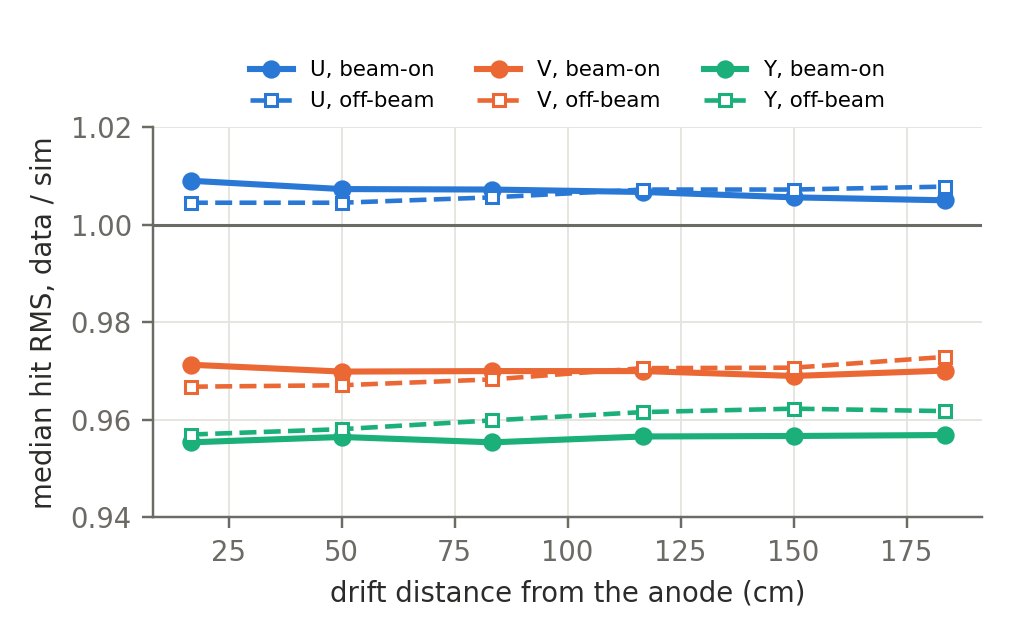
\includegraphics[width=\linewidth]{figs/width_ratio.png}\\[2pt]
      {\scriptsize median hit width, data / simulation, per plane and drift}
    \end{column}
    \begin{column}{0.50\textwidth}
      \footnotesize
      \begin{itemize}\setlength{\itemsep}{3pt}
        \item \textbf{Data vs simulation}: hits narrower in data on V ($-$3\%) and Y ($-$4.5\%), flat in drift; more low-charge Y hits;
          beam-on light $\approx$0.3\,$\mu$s later.
        \item \textbf{13 simulation-trained models vs WC} on held-out data: share of WC's $\nu$ charge also tagged \bad{0.5--0.65}
          (0.9 on simulation); at WC's off-beam rate they select 31--33\% of beam-on events, WC 45\%.
        \item \textbf{Width test (E5)}: data-like widths on simulation explain about a third of M CL's drop, none of M C+XF's.
        \item \textbf{Fixes}: data-like-width fine-tune (E6) 0.51 $\to$ 0.71; real-data fine-tune with WC labels (E7) 0.75 (not an independent check).
        \item Deck with event displays: \code{docs/sbnd-realdata-campaign.pdf}.
      \end{itemize}
    \end{column}
  \end{columns}
\end{frame}

%=====================================================================
\section{3D blobs and P3}
\begin{frame}{Why 3D, and what went into the HDF5 (\iss{15}, \iss{16})}
  \footnotesize
  \begin{columns}[T]
    \begin{column}{0.48\textwidth}
      \textbf{Wire-Cell has what qlfm lacked}
      \begin{itemize}\setlength{\itemsep}{2pt}
        \item 3D imaging: blobs from the 3 planes per time slice, charge solved with a sparsity prior;
        \item 3D clusters, and a predicted light pattern per cluster matched to the flash (Q/L matching);
        \item cosmic taggers built on these.
      \end{itemize}
      qlfm saw 2D hits per plane only, and had to learn the 2D$\to$3D geometry and charge$\to$light physics implicitly.\\[4pt]
      \textbf{Survey options} (\iss{15}): WC blobs as tokens; NuGraph-style nodes linking planes; an auxiliary 3D head; learned Q/L matching;
      sparse-CNN charge stem; OpFlash light tokens.
    \end{column}
    \begin{column}{0.50\textwidth}
      \textbf{\code{sbnd-h5maker} 0.6} (\code{prod\_aurora}, following \code{TensorSetLabeler})
      \begin{itemize}\setlength{\itemsep}{2pt}
        \item \code{wc\_blob\_table}: every blob (centre, charge, wire and slice ranges); in simulation the dominant G4 track and its share;
        \item \code{wc\_hit\_blob\_table}: hit $\leftrightarrow$ blob pairs;
        \item \code{track\_table}: per G4 track PDG, mother, start/end, momentum, $\nu$ index;
        \item \code{hit\_truth\_table}: per-hit true and SCE-displaced positions;
        \item only WC step 2 (cluster splitting) re-run on the kept step-1 outputs: $\approx$20 node-h (Aurora), $\approx$150 CPU-h (FermiGrid).
      \end{itemize}
      \textbf{Checks}: cluster ids match production exactly; 0 hit--blob pairs outside the blob; $\ge$98\% of hit charge in blobs;
      dominant-track share $\ge$0.99.
    \end{column}
  \end{columns}
\end{frame}

\begin{frame}{How well blobs give hits a 3D position}
  \footnotesize
  \begin{columns}[T]
    \begin{column}{0.50\textwidth}
      \centering\scriptsize
      per hit: blob-charge-weighted blob centre vs truth (SCE-displaced)\\[3pt]
      \begin{tabular}{lccc}
        \toprule
        & median $|\Delta x|$ & median $|\Delta y|$ & median $|\Delta z|$ \\
        \midrule
        all hits & 62--65 cm & 0.27 cm & 0.16 cm \\
        $\nu$ hits & \good{0.16 cm} & -- & -- \\
        cosmic hits & 75 cm & -- & -- \\
        \bottomrule
      \end{tabular}\\[8pt]
      \begin{tabular}{lccc}
        \toprule
        per event & simulation & beam-on & off-beam \\
        \midrule
        blobs & 4.3--4.9k & 4.4k & 4.6k \\
        blob voxel tokens (10\,cm) & 380--410 & 391 & 396 \\
        charge tokens & 1.3--1.4k & 1.46k & 1.46k \\
        hits with a 3D position & 98\% & 96\% & 96\% \\
        \bottomrule
      \end{tabular}
    \end{column}
    \begin{column}{0.48\textwidth}
      \begin{itemize}\setlength{\itemsep}{4pt}
        \item \textbf{In-time charge gets an essentially exact 3D position} (mm level in x, y, z).
        \item \textbf{Cosmics are off in x only}: blob centres are not t0-corrected, and a cosmic's arrival time is not known from charge alone.
          That is physics, not a bug: x of a cosmic needs the light.
        \item So the auxiliary 3D head predicts \textbf{y and z} (\code{--aux3d-dims yz}).
        \item Blob $\nu$ label (track $\to$ $\nu$ index) agrees with the hit truth on 99\% of the charge.
      \end{itemize}
    \end{column}
  \end{columns}
\end{frame}

\begin{frame}{The P3 model}
  \centering
  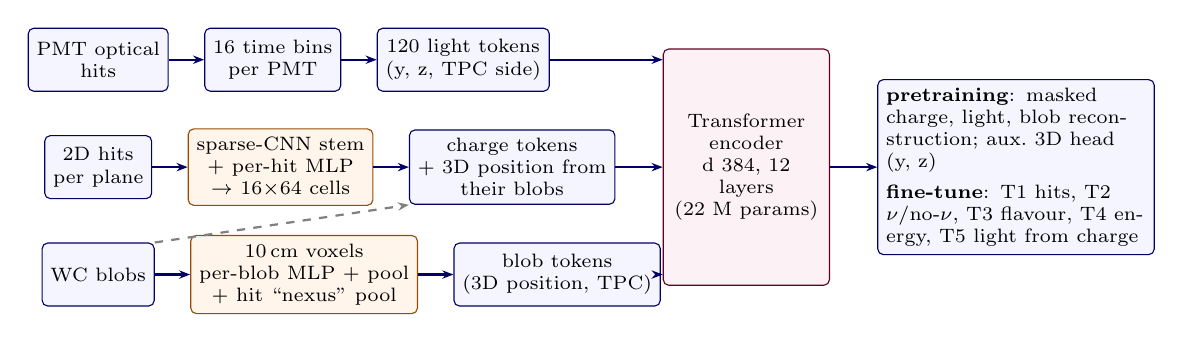
\begin{tikzpicture}[node distance=0.35cm and 0.45cm]
    \node[box] (hits) {2D hits\\per plane};
    \node[box, right=of hits, fill=orange!8, draw=orange!60!black] (stem) {sparse-CNN stem\\+ per-hit MLP\\$\to$ 16$\times$64 cells};
    \node[box, right=of stem] (ct) {charge tokens\\+ 3D position from\\their blobs};
    \node[box, below=0.55cm of hits] (blobs) {WC blobs};
    \node[box, right=of blobs, fill=orange!8, draw=orange!60!black] (vox) {10\,cm voxels\\per-blob MLP + pool\\+ hit ``nexus'' pool};
    \node[box, right=of vox] (bt) {blob tokens\\(3D position, TPC)};
    \node[box, above=0.55cm of hits] (oph) {PMT optical\\hits};
    \node[box, right=of oph] (lt0) {16 time bins\\per PMT};
    \node[box, right=of lt0] (lt) {120 light tokens\\(y, z, TPC side)};
    \node[box, right=0.6cm of ct, fill=purple!5, draw=purple!50!black, minimum height=3.0cm, text width=1.9cm] (enc) {Transformer\\encoder\\d 384, 12 layers\\(22 M params)};
    \node[box, right=0.6cm of enc, text width=3.3cm, align=left] (loss) {\textbf{pretraining}: masked charge, light, blob reconstruction;
      aux.\ 3D head (y, z)\\[3pt]\textbf{fine-tune}: T1 hits, T2 $\nu$/no-$\nu$, T3 flavour, T4 energy, T5 light from charge};
    \draw[arr] (hits) -- (stem); \draw[arr] (stem) -- (ct); \draw[arr] (blobs) -- (vox); \draw[arr] (vox) -- (bt);
    \draw[arr] (oph) -- (lt0); \draw[arr] (lt0) -- (lt);
    \draw[arr] (ct) -- (enc); \draw[arr] (bt.east) -- (enc.west |- bt.east); \draw[arr] (lt.east) -- (enc.west |- lt.east);
    \draw[arr] (enc) -- (loss);
    \draw[arr, dashed, black!50] (blobs.north east) -- (ct.south west);
  \end{tikzpicture}\\[6pt]
  \raggedright\scriptsize
  \begin{itemize}\setlength{\itemsep}{2pt}
    \item All new pieces are options (\code{--charge-stem cnn --pos3d 1 --pmt-pos v2 --blobs 1 --aux3d-weight 1}); the defaults reproduce the earlier models.
    \item No truth enters the inputs: 3D comes from WC's reconstructed blobs; blob labels are not loaded; per-hit truth is only the pretraining target.
  \end{itemize}
\end{frame}

\begin{frame}{P3 pretraining}
  \footnotesize
  \begin{columns}[T]
    \begin{column}{0.50\textwidth}
      \begin{itemize}\setlength{\itemsep}{3pt}
        \item Same recipe and events as the current SBND-pretrained M CL: 34k steps, batch 64 $\times$ 4 GPUs, 738k pretraining events
          ($\approx$12 passes).
        \item \textbf{Throughput} 757 events/s per node (current model 1,640): the model step alone allows $\approx$960; the loader was the
          bottleneck (3$\times$ more bytes per event), fixed by more workers and reading only the blob columns the model uses.
        \item \textbf{Cost} $\approx$3.2 node-h (four 1-h debug jobs).
      \end{itemize}
    \end{column}
    \begin{column}{0.48\textwidth}
      \centering\scriptsize
      final validation loss\\[3pt]
      \begin{tabular}{lcc}
        \toprule
        & P3 & current SBND M CL \\
        \midrule
        charge (masked) & \good{0.241} & 0.308 \\
        light (masked PMTs) & \good{0.407} & 0.422 \\
        light from charge only & \good{0.558} & 0.609 \\
        masked blob & 0.124 & -- \\
        auxiliary 3D (y, z) & 0.0044 & -- \\
        \bottomrule
      \end{tabular}\\[6pt]
      \raggedright\footnotesize
      Light from charge improves with 3D blob tokens: the learned version of Wire-Cell's Q/L matching.
    \end{column}
  \end{columns}
\end{frame}

%=====================================================================
\section{Results}
\begin{frame}{P3 on the SBND simulation (fine-tuned, 1\% labels, 3 seeds)}
  \centering
  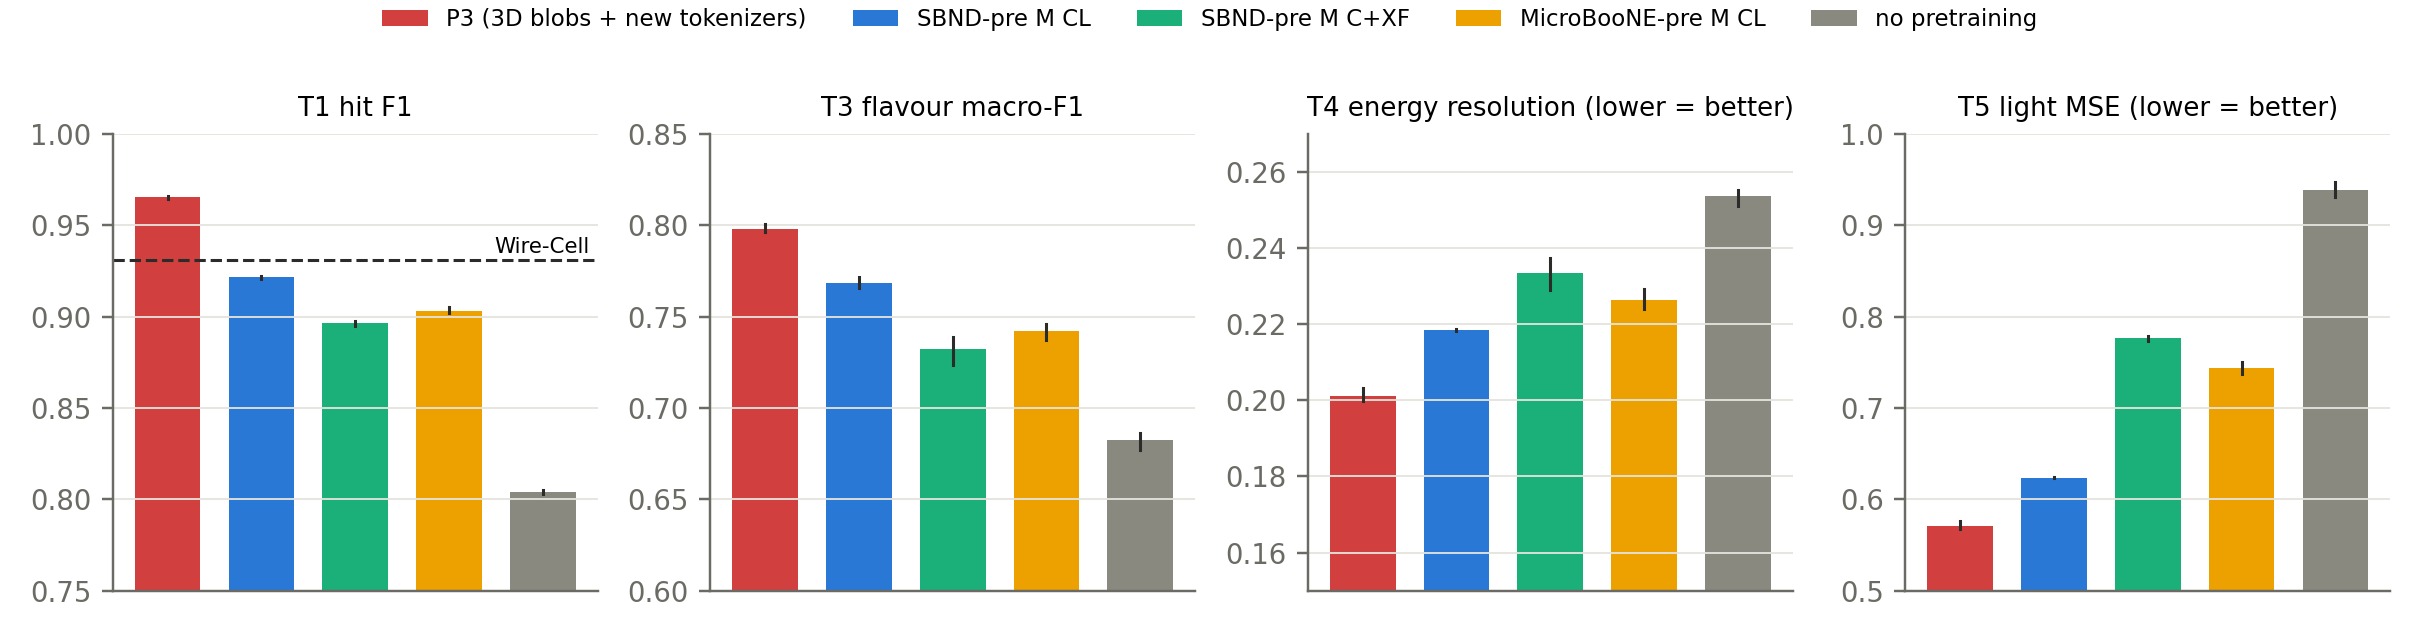
\includegraphics[width=\linewidth]{figs/p3_sim.png}\\[4pt]
  \scriptsize
  \begin{tabular}{lccccc}
    \toprule
    & T1 hit F1 & T2 AUC & T3 F1 & T4 resolution & T5 light MSE \\
    \midrule
    \textbf{P3} & \good{0.964--0.966} & \good{0.997--0.998} & \good{0.796--0.801} & \good{0.200--0.203} & \good{0.567--0.576} \\
    SBND-pre M CL (previous best) & 0.920--0.922 & 0.994--0.997 & 0.766--0.772 & 0.218--0.219 & 0.623--0.624 \\
    Wire-Cell footprint label & 0.931 & & & & \\
    \bottomrule
  \end{tabular}
\end{frame}

\begin{frame}{P3 on real data (held-out files) and the width test}
  \centering
  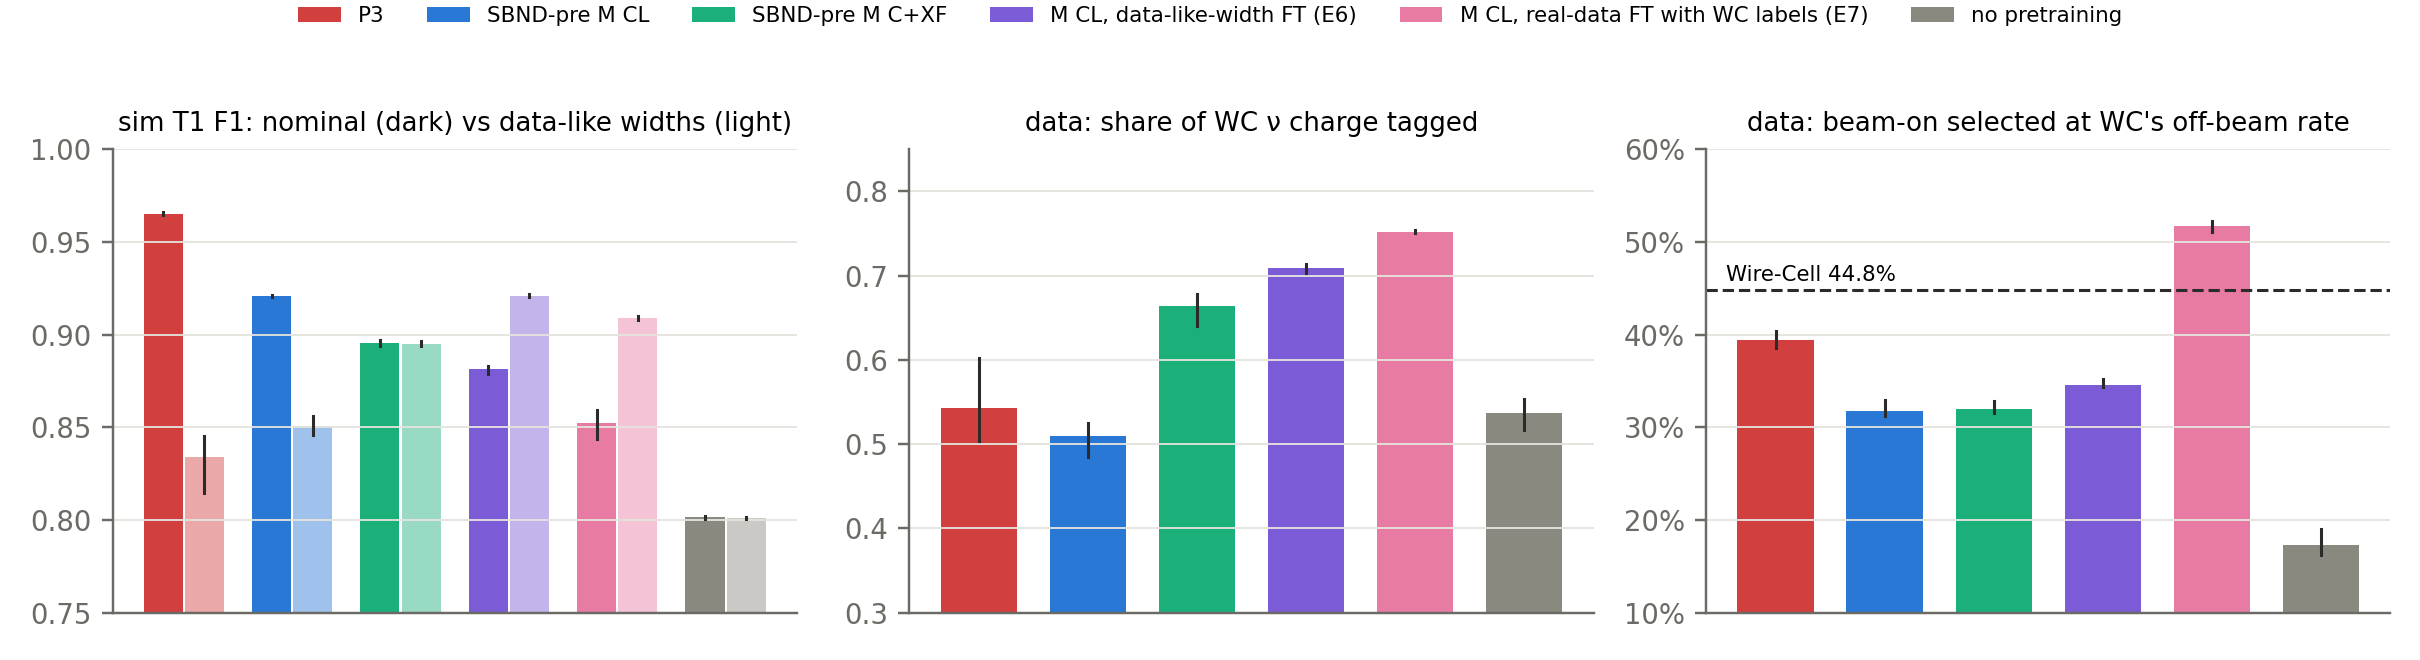
\includegraphics[width=\linewidth]{figs/p3_data.png}\\[2pt]
  \scriptsize
  \fitw{\begin{tabular}{lccccc}
    \toprule
    & sim T1, nominal / data-like widths & data: WC $\nu$ charge tagged & data: model charge in WC & beam-on selected & brightest flash in window \\
    \midrule
    \textbf{P3} & 0.965 / \bad{0.81--0.85} & 0.50--0.60 & 0.74--0.87 & \good{38.6--40.4\%} & \good{42.8--44.7\%} \\
    SBND-pre M CL & 0.921 / 0.85 & 0.49--0.53 & 0.84--0.86 & 31.2--33.0\% & 34.0--35.9\% \\
    M CL, data-like-width FT (E6) & 0.88 / 0.92 & 0.70--0.71 & 0.86--0.87 & 34.3--35.2\% & 37.6--38.7\% \\
    Wire-Cell & 0.93 & -- & -- & 44.8\% & 48.2\% \\
    \bottomrule
  \end{tabular}}\\[2pt]
  {\tiny beam-on selected: at WC's off-beam rate (6.0\%). Data: held-out 20\% of files (18,664 beam-on, 10,348 off-beam events).}
\end{frame}

\begin{frame}{Reading}
  \footnotesize
  \begin{enumerate}\setlength{\itemsep}{6pt}
    \item \textbf{3D blobs + new tokenizers help strongly in simulation.} P3 beats Wire-Cell on hit tagging and improves every task, with the
      same labels and steps as before.
    \item \textbf{Events carry over to data.} The beam-on excess over off-beam at WC's off-beam rate is now 33--34 points (previous best 25--27,
      WC 39).
    \item \textbf{Hits do not, yet.} Agreement with WC on data is 0.50--0.60 (previous 0.49--0.53), with a larger seed spread.
    \item \textbf{P3 is more width-sensitive.} With data-like widths its simulation T1 falls to 0.81--0.85, a larger drop than M CL's. The
      data/simulation width mismatch remains the main data-side limit; E6 showed that training with data-like widths fixes much of it.
  \end{enumerate}
  \vspace{4pt}
  \textbf{Caveats}
  \begin{itemize}\setlength{\itemsep}{2pt}\scriptsize
    \item On data, Wire-Cell is a reference, not truth; no exposure normalisation; both data samples are light-triggered, the simulation is not.
    \item P3 changes several things at once (CNN stem, 3D positions, blob tokens, PMT positions, 3D head): which part does what is the job of
      the ablations.
  \end{itemize}
\end{frame}

%=====================================================================
\section{Next steps}
\begin{frame}{Potential next steps}
  \tiny
  \centering
  \renewcommand{\arraystretch}{1.15}
  \begin{tabular}{c>{\raggedright\arraybackslash}p{5.9cm}>{\raggedright\arraybackslash}p{4.5cm}>{\raggedright\arraybackslash}p{2.3cm}}
    \toprule
    & step & what it answers & cost (\code{LArTPC\_FM}) \\
    \midrule
    1 & \textbf{P3 fine-tune with data-like widths} (\code{--width sbnd}, 3 seeds) & does the E6 width fix carry over to P3 on data? & $\approx$3--4 node-h \\
    2 & \textbf{P3 pretraining with randomised / data-like widths} & a width-robust backbone instead of a fine-tune fix & $\approx$3.5 node-h + fine-tunes \\
    3 & \textbf{P3 + short real-data fine-tune with WC labels} (as E7) & how far real data closes the remaining gap & $\approx$1 node-h \\
    4 & \textbf{Ablations} (former P0--P2): drop the CNN stem, the blob tokens, \code{pos3d}, the 3D head one at a time; CL vs C+XF & which part of P3 gives the gain & $\approx$3.5 node-h each \\
    5 & \textbf{Second simulation/data difference}: low-charge hits / noise and light timing (C+XF drops without width sensitivity) & what else separates data from simulation & $<$1 node-h (test-time) \\
    6 & \textbf{OpFlash light tokens and learned per-cluster Q/L matching} & does explicit flash matching help cosmic rejection & $\approx$4 node-h \\
    7 & \textbf{MicroBooNE 3D}: WC blobs from the round-1 \code{TC} trees & P3 on MicroBooNE open/real data & production work first \\
    8 & \textbf{Event displays of P3} on beam-on events where P3 and WC disagree & what the extra beam-on selections are & $<$0.1 node-h \\
    \bottomrule
  \end{tabular}\\[6pt]
  \raggedright\footnotesize
  \textbf{Suggested order}: 1 and 8 now (cheap, directly address the data-side gap); 4 (ablations) for the paper; 2 or 3 depending on 1.
\end{frame}

%=====================================================================
\begin{frame}{Backup: compute, storage, code}
  \scriptsize
  \begin{itemize}\setlength{\itemsep}{3pt}
    \item \textbf{Polaris compute on \code{LArTPC\_FM}} for P3: pretraining $\approx$3.2 node-h, fine-tunes $\approx$2, evaluations $\approx$0.5, cache work and
      tests $<$1. SBND real-data campaign (E3--E7) $\approx$4 node-h. Aurora 0.6 simulation $\approx$20 node-h; FermiGrid 0.6 data $\approx$150 CPU-h.
    \item \textbf{Storage}: \code{/lus/eagle/projects/LArTPC\_FM/yuhw/} (20 TB quota): \code{fm4npp-lartpc-data/sbnd-*/v06}, \code{fm4npp-lartpc-work/cache/sbnd\_m},
      \code{sbnd\_data\_m}, P3 models in \code{fm4npp-lartpc-work/p3/}.
    \item \textbf{Code} (main): tokenizers and model options ad2ed66; converter for 0.6 3aeb248; in-place cache update 1b7d24e; loader fix 115d154;
      \code{sbnd-h5maker} 0.6 3cdad6b / 8f31637.
    \item \textbf{Docs}: \code{docs/survey-3d-tokenizers.md}, \code{docs/plan-3d-blobs.md}, \code{docs/sbnd-realdata-campaign.pdf}.
    \item \textbf{Results}: \code{fm4npp-lartpc-work/sbnd\_data/eval/report\_p3.json}, \code{report\_all.jsonl}; fine-tune metrics in \code{p3/ft/f0.01\_s*}.
  \end{itemize}
\end{frame}

\end{document}
